Consider the classical example of balancing an inversed pendulum on a cart by applying a series of forces to the cart. The \emph{environment} at a given time-step $t$ is represented by the state $\nvec{s}_t = \begin{smallmatrix} \begin{bmatrix} x_{t} & \dot{x}_{t} & \varphi_{t} & \dot{\varphi}_{t} \end{bmatrix}^T \end{smallmatrix}$, where the variables $x_{t}$, $\dot{x}_{t}$, $\varphi_{t}$, and $\dot{\varphi}_{t}$ denote the cart's position, and cart's velocity in the $x$-direction, the pendulum's angle with respect to the vertical, and the pendulum's angular velocity, at the time-step $t$, respectively. The available choices of action $a \in \mathcal{A} = \left\{ -F \ +F \right\}$ are applying a constant force $F$ to the cart in either the right or left direction. According to the performed action $a_{t} = {\policy}(\nvec{s}_t)$, the environmental state evolves to the next state $\nvec{s}_{t+1}$, as governed by the dynamical equations of the cart and pendulum as shown in (\ref{eq:AngularAccCartPole}) and (\ref{eq:AccCartPole}). Frictional effects are neglected for the sake of simplicity.
\begin{equation}
    \begin{split}
    \ddot{\varphi}_{t} &= \frac{a_t \cos{{\varphi}_t} + m_p \dot{{\varphi}_t}^2 \ell \sin{{\varphi}_t} \cos{{\varphi}_t} - (m_c + m_p)g\sin{{\varphi}_t}}
                         { \dfrac{4}{3} \ell (m_c + m_p) - m_p \ell \cos{{\varphi}_t}^2} \,, \\
    a_t &= 
    \begin{cases}
      +F & \text{force F applied to the right of the cart} \\
      -F & \text{force F applied to the left of the cart}           
    \end{cases}
    \end{split}
    \label{eq:AngularAccCartPole}
\end{equation}
\begin{equation}
    \ddot{x}_{t} = \frac{1}{\cos{{\varphi}_t}} \left[ \dfrac{4}{3} \ell \ddot{{\varphi}_t} + g\sin{{\varphi}_t} \right]
    \label{eq:AccCartPole}
\end{equation}
The mass of the cart is denoted by $m_c$, and the pendulum modelled by a massless rod of length $\ell$, with a point mass $m_p$ fixed on one end as shown Figure \ref{fig:RLSchematic}, while the other end is in turn attached to the cart by a revolute joint. Applying for instance, the Euler method over a step size $\Delta t$, the next state $\nvec{s}_{t+1}$ is obtained as shown in (\ref{eq:EulerIntegrationCartPole})
\begin{equation}
    \nvec{s}_{t+1} =
    \begin{bmatrix}
        x_{t+1} \\ \dot{x}_{t+1} \\ \varphi_{t+1} \\ \dot{\varphi}_{t+1}
    \end{bmatrix} =
    \begin{bmatrix}
        x_{t} + \dot{x}_{t} \cdot \Delta t\\
        \dot{x}_{t} + \ddot{x}_{t} \cdot \Delta t\\
        \varphi_{t} + \dot{\varphi}_{t} \cdot \Delta t\\
        \dot{\varphi}_{t} + \ddot{\varphi}_{t} \cdot \Delta t
    \end{bmatrix} \,.
    \label{eq:EulerIntegrationCartPole}
\end{equation}
The reward function is defined as shown in (\ref{eq:RewardFunctionCartPole})
\begin{equation}
  R(\nvec{s}_{t+1}) =
  \begin{cases}
    +1 & \text{if } |{\varphi}_{t+1}| < \varphi^* \\
    0 & \text{if } |{\varphi}_{t+1}| \geq \varphi^*
  \end{cases} \,,
  \label{eq:RewardFunctionCartPole}
\end{equation}
and the termination condition in (\ref{eq:TerminationConditionCartPole})
\begin{equation}
  T_{\text{end}} =
  \left\{
  \begin{array}{rll}
    \text{true} & \text{if } |{\varphi}_{t+1}| \geq \varphi^* & \text{(pendulum falls over)} \\
    \text{true} & \text{if } |{x}_{t+1}| \geq x^* & \text{(positional limit of cart due to physical constraints)} \\
    \text{true} & \text{if } t = 500 & \text{(end simulation due to time-constraint)} \\
    \text{false} & \text{otherwise} & \text{(pendulum kept balanced)}
  \end{array}
  \right. \,,
  \label{eq:TerminationConditionCartPole}
\end{equation}
where $\varphi^*$ and $x^*$ denote thresholds for the angle of the pendulum with respect to the vertical and position of the cart in the $x$-direction, respectively. The DQL algorithm has since been adapted to develop other algorithms such as the Deep Deterministic Policy Gradient algorithm by \cite{lillicrap2015}, which allows for continuous (real-valued) and high-dimensional action spaces.

To implement this example, the environmental parameters, as well as the DQL agent hyperparameters are initialized with values as shown in Table \ref{tab:CartPoleParameters}. The policy and target networks were implemented as multilayer perceptron (MLP) with two hidden layers, each with 128 neurons. The agent is then subsequently trained according to Algorithm \ref{alg:DQN} over 750 episodes, where the parameters $\boldsymbol{\theta}$ of the $Q$-network are optimized using an AdamW optimizer \cite{loshchilov2017}, with the learning rate $l_r$. The learning was carried out on a 5.3 GHz Intel\textsuperscript{\textregistered{}} Core\texttrademark{} i9-10900K CPU, and implemented with the deep learning framework PyTorch \cite{pytorch}, as well as other libraries for applications in science and data analysis (e.g. pandas \cite{pandas}, SciPy \cite{scipy}, NumPy \cite{numpy}) in the Python programming language.

As shown in Figure \ref{fig:PendulumDuration}, the duration (i.e. total time-steps) of the pendulum kept balanced increases over the course of training and even ultimately reaches the maximum permitted number of time-steps as set in (\ref{eq:TerminationConditionCartPole}). One can also observe how the agent progressively improves, and its learning eventually converges to an optimal policy $\optpolicy$, as implied in Figure \ref{fig:QValuesProgression} with the converging $Q$-Values. 
\begin{table}[H]
  \centering
  \begin{tabular}{p{0.65\textwidth}p{0.055\textwidth}p{0.1\textwidth}}
    \hline
    \multicolumn{3}{l}{\textbf{Environmental Parameters}} \\
    \hline
    Mass of cart & $m_c$ & 1.0 \si{kg} \\
    Mass of point mass on end of pole & $m_p$ & 0.1 \si{kg} \\
    Length of pole & $\ell$ & 1.0 \si{m} \\
    Magnitude of force applied to cart in $x$-direction & $F$ & 10 \si{N} \\
    Gravitational acceleration & $g$ & 9.8 \si{m/s^2} \\
    Threshold angle with respect to vertical  & $\varphi^*$ & \ang{12} \\
    Threshold position of cart in $x$-direciton  & $x^*$ & 2.4 \si{m} \\
    Step size & $\Delta t$ & 0.02 \si{s} \\
    \hline
    \multicolumn{3}{l}{\textbf{Agent Hyperparameters}} \\
    \hline
    Number of episodes & $K$ & 750 \\
    Number of experiences stored in replay memory & $N$ & 10000 \\
    Discount rate & $\gamma$ & 0.99 \\
    Batch size of experiences drawn from replay memory & $|\mathcal{B}_{D}|$ & 128 \\
    Learning rate of AdamW optimizer & $l_r$ & \num{1e-4} \\
    Soft target update rate & $\tau$ & 0.005 \\
    Initial probability $\epsilon$ for random exploration & $\epsilon_{\text{initial}}$ & 0.9 \\
    Final probability $\epsilon$ for random exploration & $\epsilon_{\text{final}}$ & 0.05 \\
    Decay rate of probability $\epsilon$ for random exploration & $\epsilon_{\text{decay}}$ & 1000 \\
    \hline
  \end{tabular}
  \caption{Environmental parameters for the example of balancing an inversed pendulum on a cart, and the learning hyperparameters of the DQL agent.}
  \label{tab:CartPoleParameters}
\end{table}
\begin{figure}[H]
  \centering
  \vspace{-1.0em}
  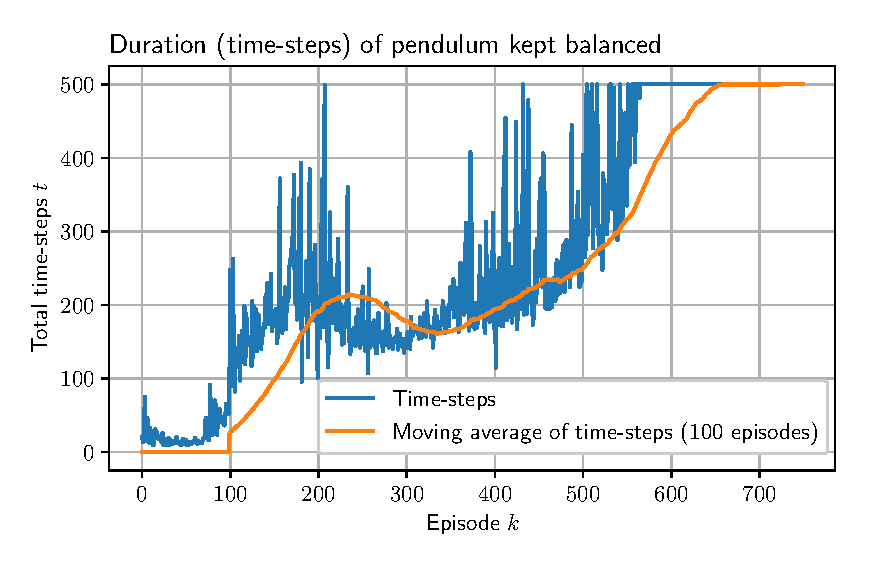
\includegraphics[width=1.0\textwidth]{PendulumDuration}
  % Matptlotlib Customized Settings
  % figsize=(6.25, 3.5)
  % loc='left', fontsize='large'
  \vspace{-1.5em}
  \caption{Duration of pendulum kept upright over training episodes.}
  \label{fig:PendulumDuration}
\end{figure}
% \begin{figure}[H]
%   \centering
%   \vspace{-1.0em}
%   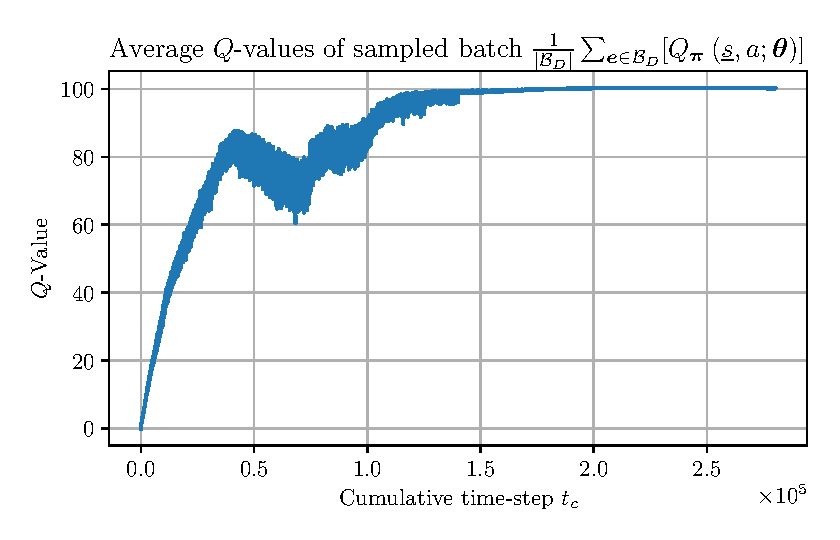
\includegraphics[width=1.0\textwidth]{QValuesPendulum}
%   % Matptlotlib Customized Settings
%   % figsize=(5.5, 3.5)
%   % ax.ticklabel_format(style='sci', axis='x', scilimits=(0,0))
%   % loc='left', fontsize='large
%   \vspace{-1.5em}
%   \caption{Progression of $Q$-values over the course of training.}
%   \label{fig:QValuesProgression}
% \end{figure}
